\chapter{Results and Discussion}
The results presented here concern the effective three-body potential curves obtained by solving \Cref{adiabatic} within the strict adiabatic treatment, see \Cref{sec:Effective_3B}. Signatures of the Efimov effect can be revealed in the structure of these adiabatic hyperspherical potentials, with the Efimov channel corresponding to the one emergent attractive potential converging to \eqref{eq:efimov_channel} in the region $r_0 \ll \rho \ll
\abs{a}$.

The adiabatic potential curves were obtained by numerically solving \Cref{adiabatic} in  two-dimensional hyperangular space at fixed hyperradii using the method outlined in \Cref{chapter:5}. The two-body scattering model described in \Cref{chapter:scattering_model} was used with the interaction range fixed at $r_0=55$ a.u. and with masses corresponding to the bosonic rubidium isotope $m = m( \prescript{87}{}{\mathrm{Rb}})$. 

We expect the potential curves to converge towards \eqref{eq:efimov_channel} for $\abs{a} \rightarrow \infty$. This behaviour is more easily recognized if the potentials are multiplied by $2 \mu \rho^2$ and plotted as 

\begin{equation}\label{eq:lambda}
\xi(\rho) = 2 \mu \rho^2 W_{\nu}(\rho) + \frac{1}{4},
\end{equation}
since these curves should approach the universal value $-s_0^2 (\simeq -1.0125$ for $J=0^+$ states) for the lowest effective potential. This scenario is restricted to the range $r_0 \ll \rho \ll \abs{a}$ and we only expect to find a potential $\xi(\rho)$ that is infinitely extended towards this universal value in the resonant regime when the magnitude of the scattering length is infinite. In this regime, the solution $\xi_{\infty}(\rho/\abs{a}) = -s_0^2$ gives rise to an effective attractive potential, which is proportional to $\rho^{-2}$. This effective attractive potential is substituted into the hyperradial equation \eqref{fullhamiltonian}, where it in turn results in an infinite number of bound trimer states.

We start by exploring Efimov's original scenario for two effective potentials calculated with two-body interactions very close to the resonant regime $a \approx \pm \infty$. The values of the potential depths $d$ were tuned near the pole labelled $\mathrm{I}$ in \Cref{fig:res_1}, so that the two-body potential was just short of, or could just barely, support a single two-body bound state. To confirm the validity of the code the convergence of the adiabatic eigenvalues was tested over a broad range of hyperradii $\rho$ using an increasing number of B-splines in each hypersperical dimension. 

In \Cref{table:Res_2} we present a systematic analysis of the numerical potential values $\xi(\rho)$ for the two cases where the scattering length was tuned to $a_1 \rightarrow -\infty$ and $a_2 \rightarrow \infty$. The adiabatic eigenvalues were calculated at ten different hyperradial points using $40$, $60$, $80$ and $100$ B-splines in each coordinate dimension. The convergence of our numerical potentials for values of $\rho$ up to $\rho_{max} = 2 \times 10^4$ a.u. is indictated by the fact that the numerical values for the effective three-body potential energies are virtually unaffected by increasing the number of B-splines past $N_{\theta}=80$. We also observe numerical convergence towards the universal constant $-s_0^2$ for $\rho \approx 1.5 \times 10^4$ a.u. 

In \Cref{fig:infty} we show the results obtained over the full hyperradial range up to $2 \times 10^4$ a.u., where the numerically calculated effective three-body potentials $\xi(\rho)$ are plotted as functions of $\rho$. Note the logarithmic scale on the hyperradial axis. The curves can here be seen to converge towards the characteristic universal value $-s_0^2$ for $\rho \gg r_0$. 

\begin{table}[h!]
	\centering
	\footnotesize
	\begin{adjustwidth}{-0.1cm}{}
		\tabcolsep=0.10cm
		\begin{tabular}{||c c c c c c c||} 
			\hline
			$a$ (a.u.) & $N_{\theta}$ & $\xi(\rho = 10 $ a.u.) & $\xi(100 $ a.u.) & $\xi(1000 $ a.u.) & $\xi(5000 $ a.u.) & $\xi(10000 $ a.u.)  \Tstrut\Bstrut \\ [0.7ex]
			\hline\hline  \Tstrut\Bstrut 
			$a_1$   & 40  & 3.77527814 & $-$2.60368386 & $-$1.13917612 & $-$1.03381589& $-$1.01875933 \\
			$a_1$   & 60  & 3.77527814 & $-$2.60368386 & $-$1.13917794 & $-$1.03402415& $-$1.01912287\\
			$a_1$   & 80  & 3.77527828 & $-$2.60368371 & $-$1.139177577 & $-$1.03402813 & $-$1.01913547 \\
			$a_1$   & 100  & 3.77530687 & $-$2.60367681 & $-$1.13917744 & $-$1.03405123 & $-$1.01907622 \\ [0.5ex]
			\hline \Tstrut\Bstrut 
			$a_2$   & 40  & 3.77526186 & $-$2.60416378 & $-$1.14059415 & $-$1.04035560 & $-$1.03170805 \\
			$a_2$   & 60  & 3.77526186 & $-$2.60416378 & $-$1.14058505 & $-$1.04056429 & $-$1.03207318 \\
			$a_2$   & 80  & 3.77526201 & $-$2.60416363 & $-$1.14059531 & $-$1.04056828 & $-$1.03208587 \\
			$a_2$   & 100  & 3.77526909 & $-$2.60416169 & $-$1.14059543 & $-$1.04056460 & $-$1.03224689 \\ [0.7ex] 
			\hline
			\hline
			$a$ (a.u.) & $N_{\theta}$ & $\xi(14900 $ a.u.) & $\xi(15000 $ a.u.) & $\xi(16000 $ a.u.) & $\xi(18000 $ a.u.) & $\xi(20000 $ a.u.)  \Tstrut\Bstrut \\ [0.7ex]
			\hline\hline  \Tstrut\Bstrut 
			$a_1$   & 40  & $-$1.01212794 & $-$1.01201907 & $-$1.01096343 & $-$1.00898721& $-$1.00713887 \\
			$a_1$   & 60  & $-$1.01250001& $-$1.01239204 & $-$1.01134994 & $-$1.00943386 & $-$1.00768456 \\
			$a_1$   & 80 & $-$1.01251258 & $-$1.01240462 & $-$1.01136252 & $-$1.00944702 & $-$1.00770029 \\
			$a_1$   & 100  & $-$1.01252039 & $-$1.01240590 & $-$1.01136323 & $-$1.00944483& $-$1.00769735 \\[0.5ex]
			\hline  \Tstrut\Bstrut 
			$a_2$   & 40 & $-$1.03136024 & $-$1.03137963 & $-$1.03160655 & $-$1.03219548 & $-$1.03291215 \\
			$a_2$   & 60 & $-$1.03173468 & $-$1.03175498 & $-$1.03199569 & $-$1.03264543 & $-$1.03346237 \\
			$a_2$   & 80  & $-$1.03174732 & $-$1.03176768 & $-$1.03200835 & $-$1.03265877 & $-$1.03347809 \\
			$a_2$   & 100 & $-$1.03174824 & $-$1.03176640 & $-$1.03200772 & $-$1.03265632 & $-$1.03347885 \\ [0.7ex] 
			\hline
		\end{tabular}
	\end{adjustwidth}
	\caption{Effective three-body potential values $\xi(\rho)$ at different hyperradii for $a_1 = -2702020$ a.u. $a_1 = 1966590$ a.u. The potential for $a<0$ have converged, while the potential for $a>0$ tends to converge to the universal value $-s_0^2 \simeq -1.01251$ at the hyperradii close to $\rho=15000$ a.u.}
	\label{table:Res_2}
\end{table} 

\begin{figure}
	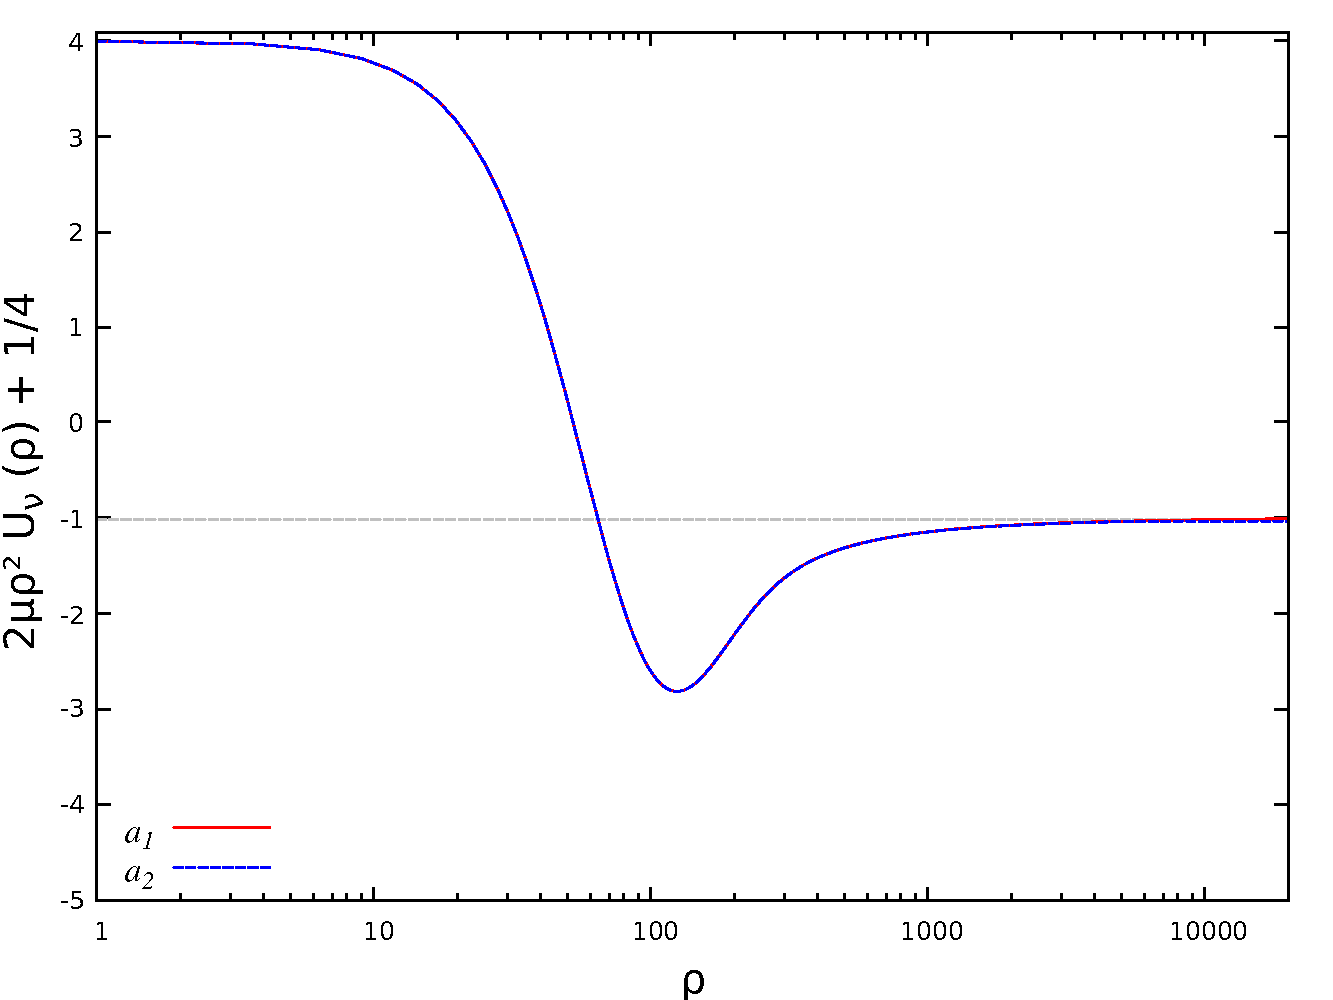
\includegraphics[width=\linewidth]{infty.pdf}
	\caption{The lowest three-body effective potential curves $\xi(\rho)$ are plotted as functions of $\rho$ for $a_1 = -2702020$ a.u. $a_1 = 1966590$ a.u. over the full range of hyperradii for which the numerically calculated potentials converged.}
	\label{fig:infty}
\end{figure}

Next, we consider the near-resonant scenario for finite $a$. For short-ranged two-body potentials where the magnitude of the scattering length is large but finite we expect that the effective potentials $W_{\nu}(\rho)$ are to some extent affected by Efimov physics in the range $r_0 \ll \rho \ll \abs{a}$ and that the lowest effective potentials obtained with a larger magnitude of $a$ exhibit closer resemblence with the true Efimov potential given in \Cref{eq:lambda}. However, in the asymptotic limit $\rho \rightarrow \infty$, when $\rho \ll \abs{a}$ is not fulfilled, we anticipate that the behaviour of $W_{\nu}(\rho)$ depends on the sign of $a$, since it indicates whether or not the two-body interaction is strong enough to support a binary state and henceforth indicates the associated break-up channel. For $a>0$ the effective potentials $W_{\nu}(\rho)$ are expected to converge asymptotically to the energy of the weakly bound dimer \eqref{eq:weakdimer}. For $a<0$ we instead expect that the effective potentials $W_{\nu}(\rho)$ asymptotically approach \eqref{eq:continuumchannel}, i.e., the eigenvalues of the kinetic energy, which for the lowest potential $\xi(\rho)$ corresponds to $\lambda(\lambda + 4) + 4$ with $\lambda = 0$.

In \Cref{fig:res_5} the potential curves for $a>0$, asymptotically associated with the weakly bound dimer channel $\nu = 0$, are plotted as functions of the hyperradius $\rho$ for four different values of $a$. The results presented in this figure were obtained using values of $d$ that approached pole $\mathrm{I}$ from the right, thus supporting a single two-body bound state. The Efimov-like character of the effective three-body potentials is manifested by the flattening behaviour of the curves over an extended region in the intermediate range $r_0 \ll \rho \ll |a|$, which tend to converge towards the universal value $-s_0^2$ (indicated in the figure by the horizontal dashed line), as the magnitude of the scattering length is gradually increased. The asymptotic convergence of the effective potentials $W_{\nu}(\rho)$ to the channel of one weakly bound dimer and a free atom can in this figure be recognized by $\xi(\rho)$ displaying a parabolic dependence of $\rho$ in the asymptotic limit for each state. We highlight this behaviour for the two effective potentials obtained with the smallest values of $a$ in \Cref{fig:finite_conv} by including the two asymptotic forms $\xi_+ = 2\mu \rho^2 E_{2b} + 1/4$, calculated from the two-body energy $E_{2b}$ given in \Cref{eq:exact_2b}.   

\begin{figure}
	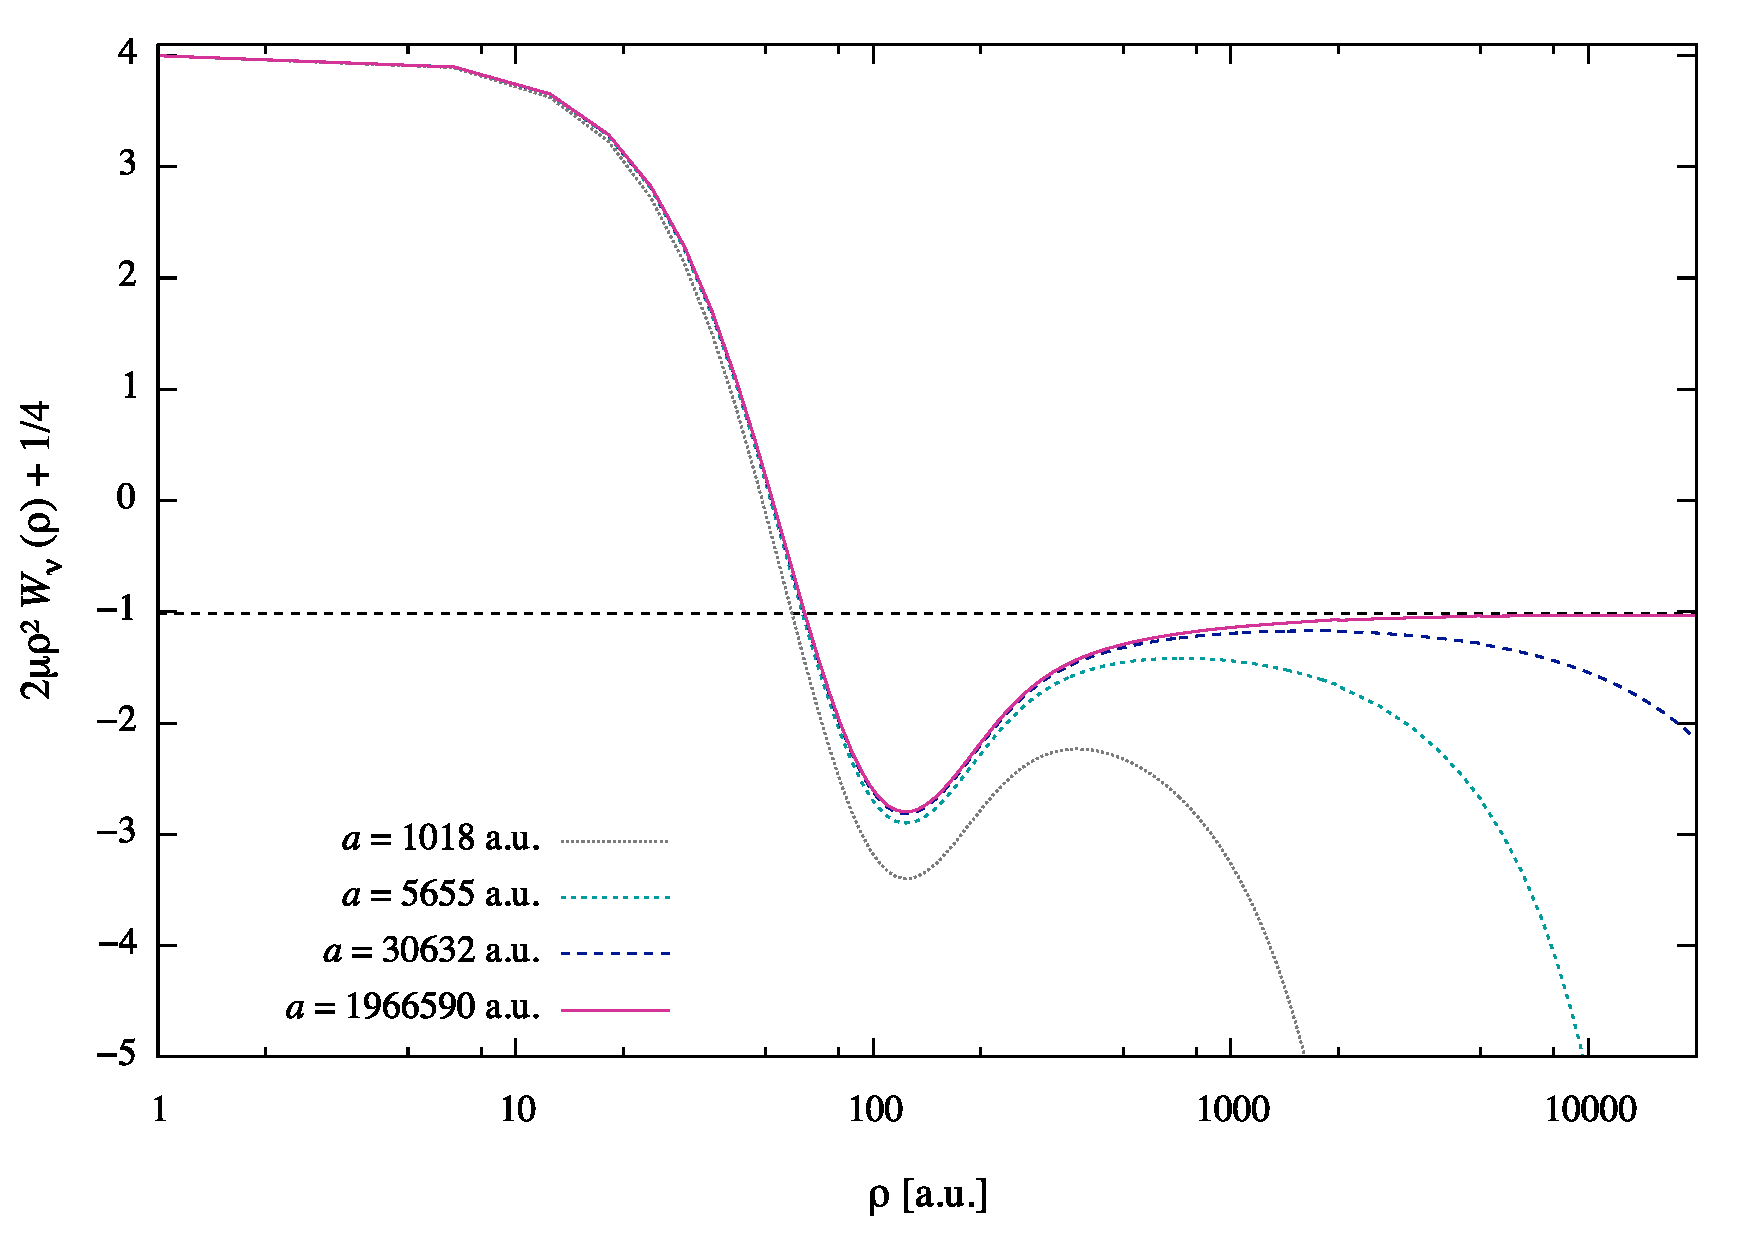
\includegraphics[width=\linewidth]{finite_positive_a.pdf}
	\caption{Effective three-body potentials for $a>0$. The horizontal dashed line is $-s_0^2$.}
	\label{fig:res_5}
\end{figure}

\begin{figure}
	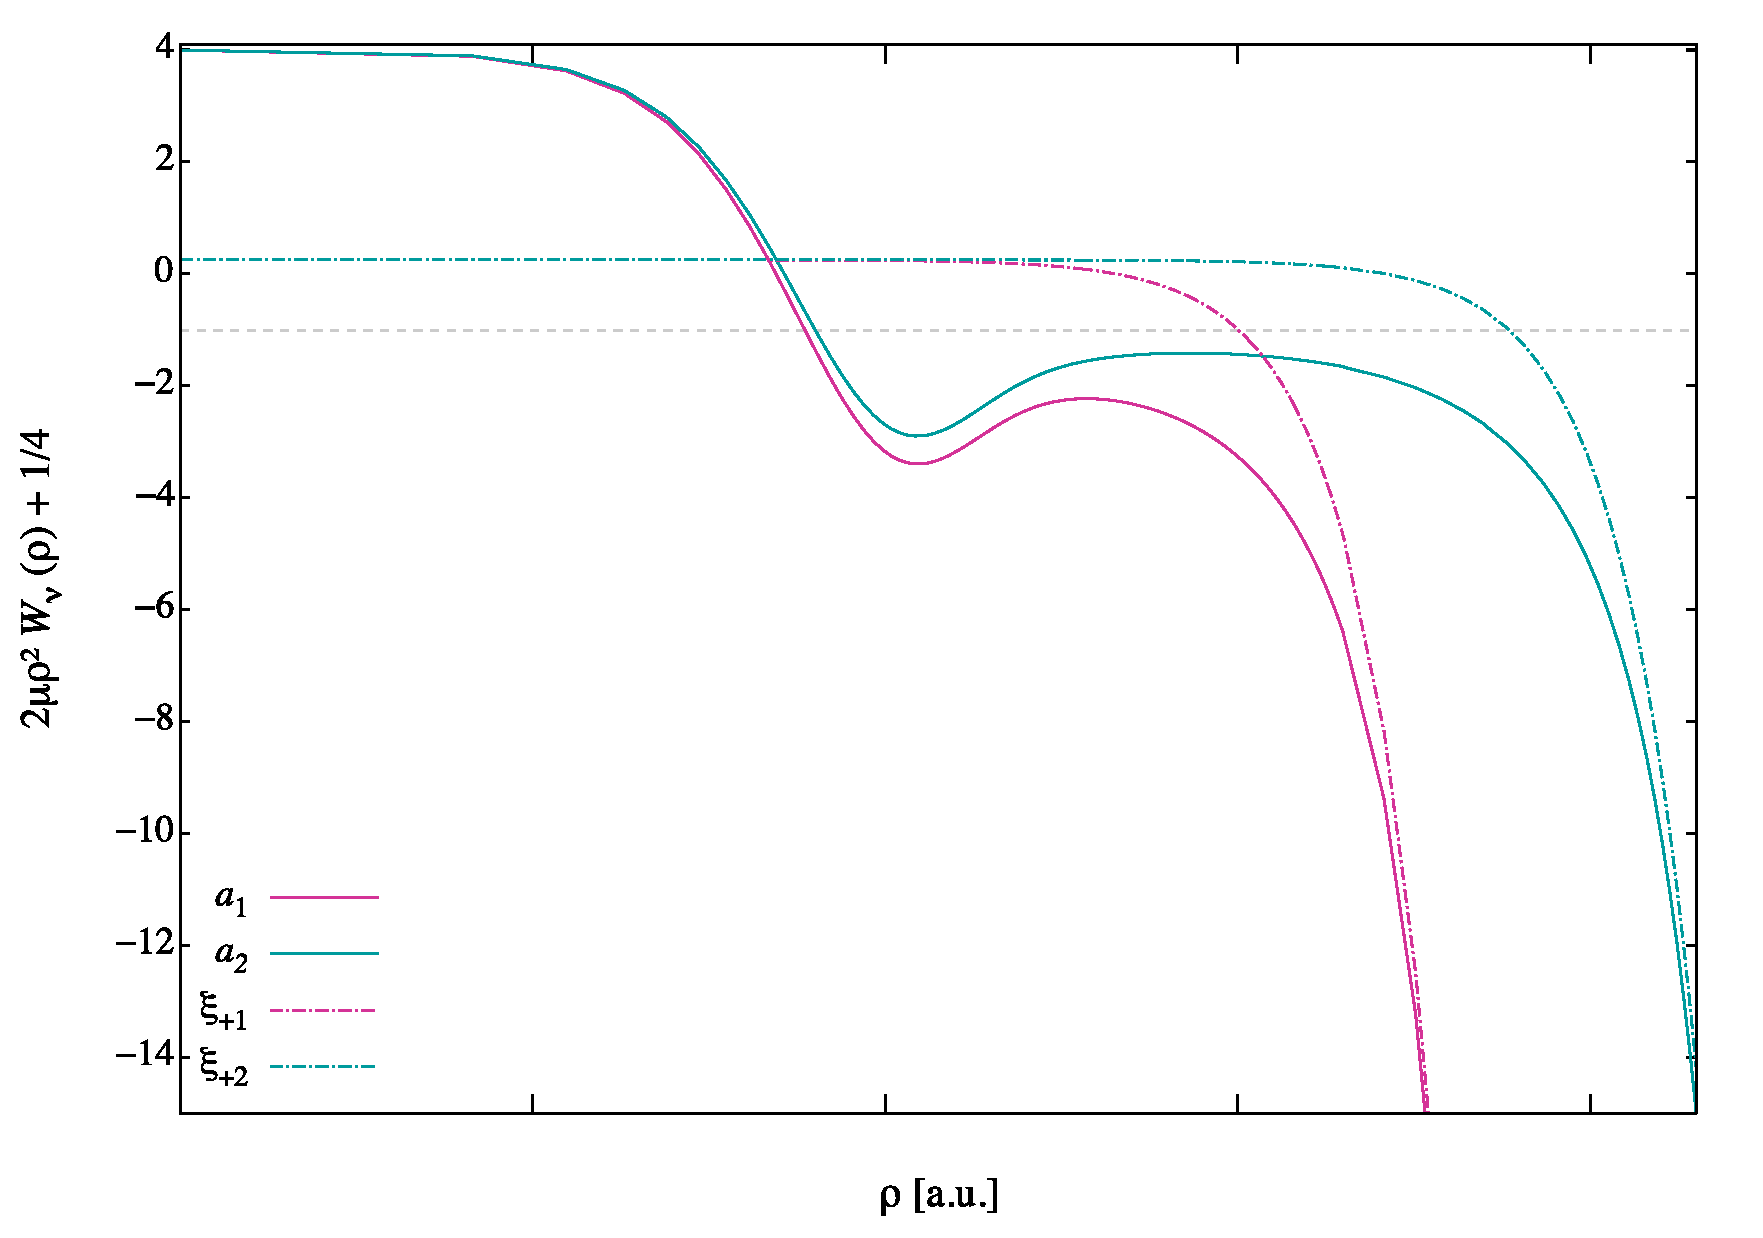
\includegraphics[width=\linewidth]{finite_conv.pdf}
	\caption{The effective three-body potentials for $a_1=1018$ a.u. and $a_2=5655$ a.u. are highlighted and showed together with their analytical asymptotic forms $\xi_{+1}$ and $\xi_{+2}$.}
	\label{fig:finite_conv}
\end{figure}

In \Cref{fig:res_3} the potential curves for $a<0$, asymptotically associated with the lowest continuum channel, are plotted as functions of the hyperradius $\rho$ for four different values of $a$. These effective three-body potentials also exhibit Efimov-like characteristics in the range $r_0 \ll \rho \ll |a|$, which can be discerned from the tendency of the potential curves to converge to $-s_0^2$ as the magnitude of $a$ increases, while they return to the kinetic energy in the asymptotic limit.

\begin{figure}
	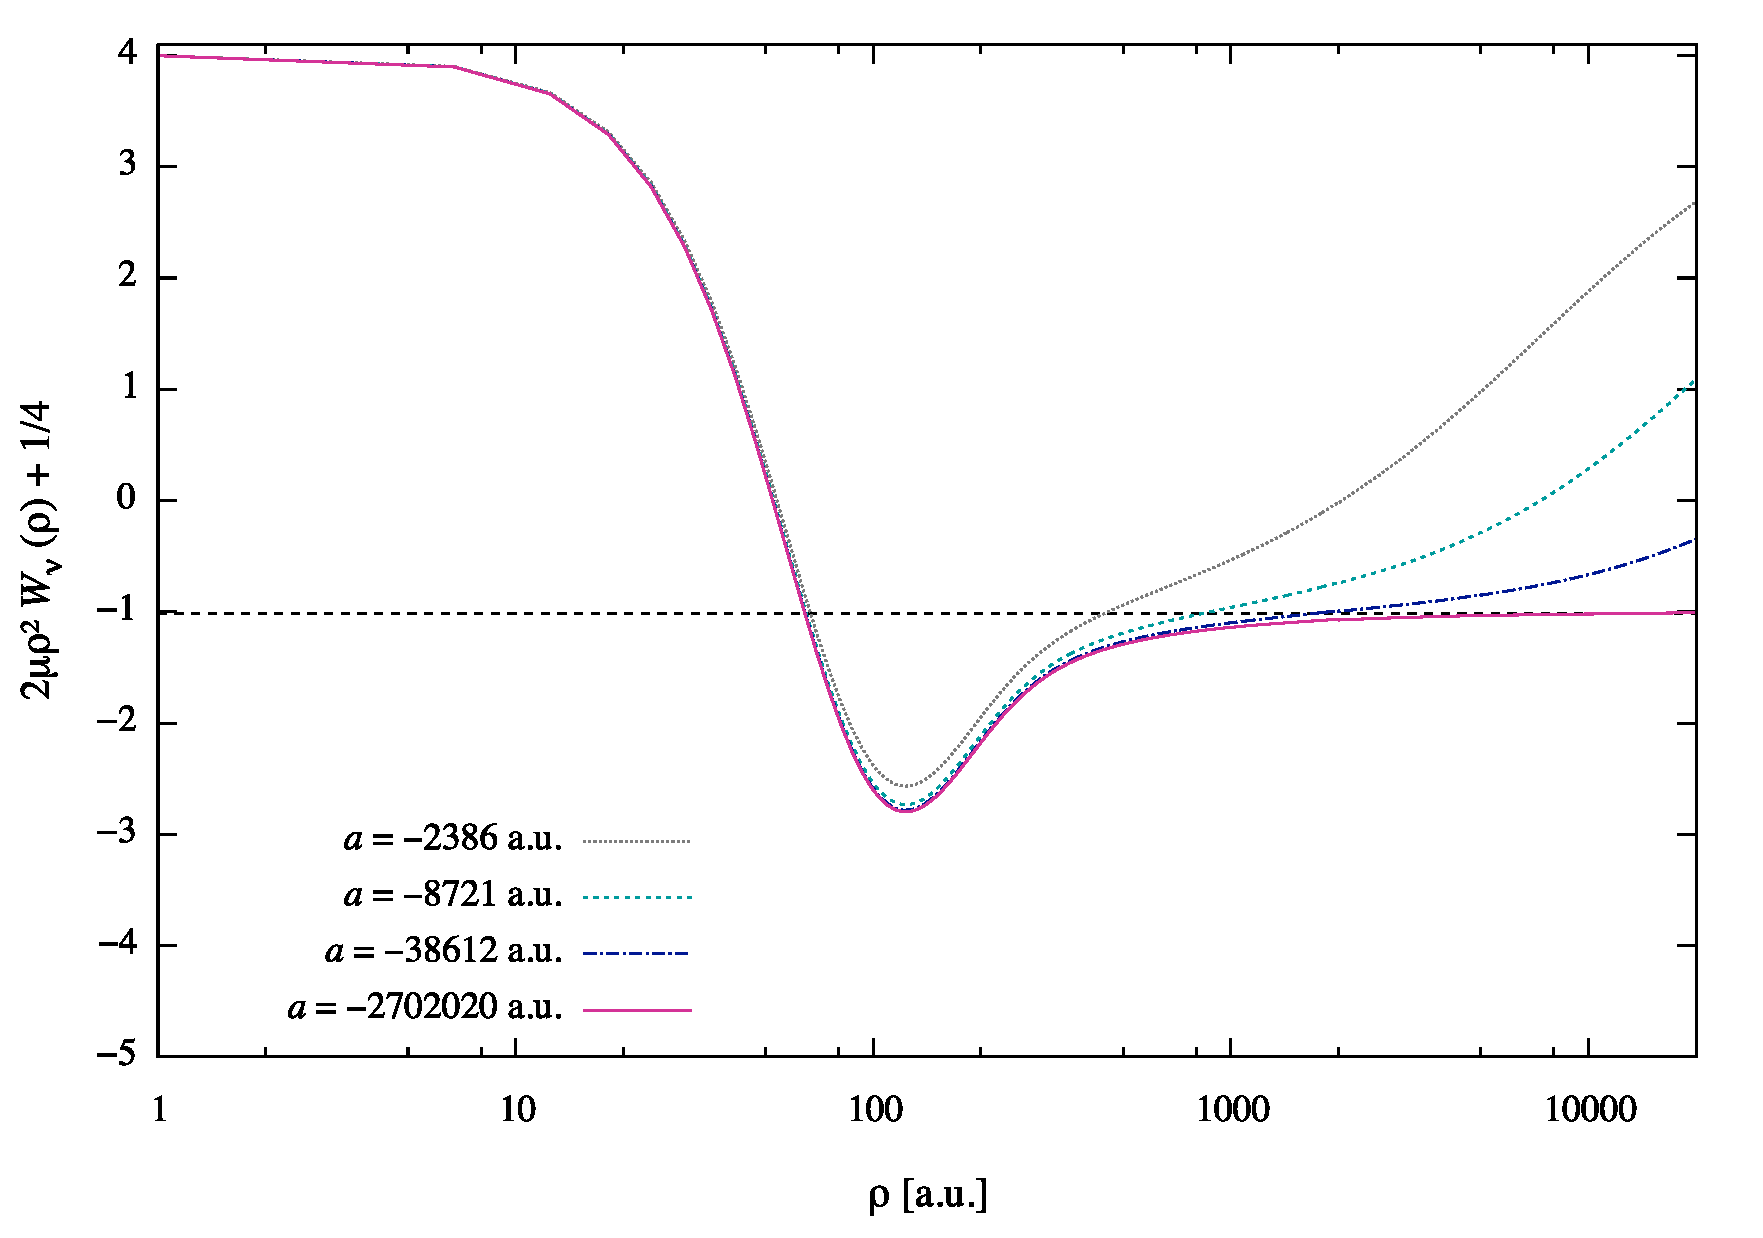
\includegraphics[width=\linewidth]{finite_negative_a.pdf}
	\caption{Effective three-body potentials for $a<0$. The horizontal dashed line is the value $-s_0^2$, which the Efimov potential takes on for $\rho\gg r_0$.}
	\label{fig:res_3}
\end{figure}

To further investigate the validity of the code we now compare our numerically calculated effective three-body potentials $\xi(\rho)$ for a number of finite $a$ states, with the lowest energy eigenvalues $\nu_n(\rho)$ of the adiabatic hyperangular Faddeev equation for $a>0$ and $a<0$. These eigenvalues can be derived analytically in the limit of large $\abs{a}$ over the full hyperradial range and are determined by solving the transcendental equation \eqref{eq:transcendental}. The adiabatic eigenvalues $\nu_n(\rho)$ of \Cref{eq:faddeev_hyperang} are related to the effective three-body potentials calculated in this work through \Cref{eq:faddeev_effectivepot}. 

In \Cref{fig:faddeev} we present the lowest eigenvalues $\nu_0(\rho/\abs{a})$ calculated from \Cref{eq:transcendental} for $a>0$ and $a<0$. For both positive and negative $a$, the adiabatic states converge to the universal value $\nu_0(0) = -s_0^2$ in the region where $\rho/\abs{a}$ is small. For large $\rho/\abs{a}$, however, we observe that $\nu_0(\rho/\abs{a})$ for $a>0$ takes on a parabolic asymptotic form, which corresponds to a state with one diatomic molecule and one free atom, whereas for $a<0$ the state can be seen to approach $\nu_0=4$, thus corresponding to the lowest kinetic energy eigenvalue for three free atoms.  

\begin{figure}
	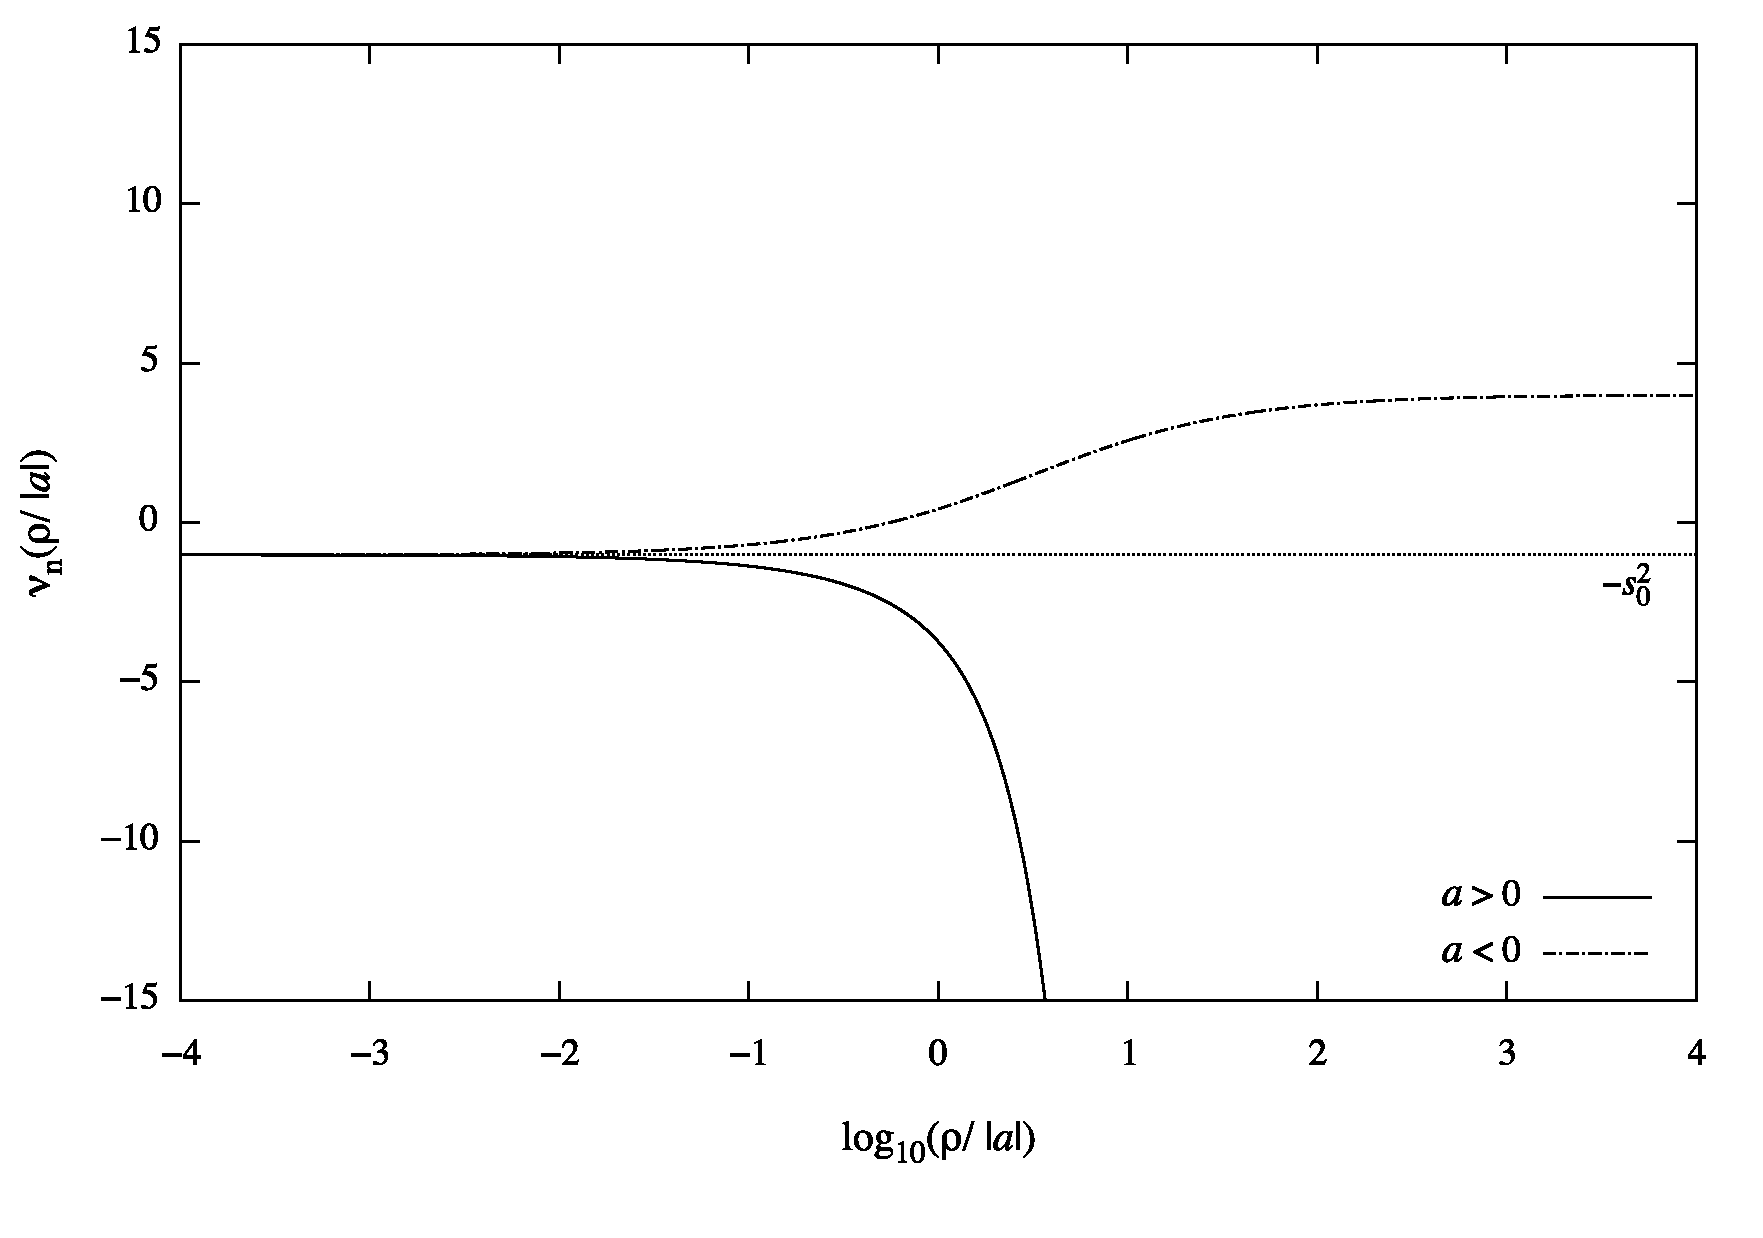
\includegraphics[width=\linewidth]{faddeev.pdf}
	\caption{Eigenvalues $\nu_0(\rho/\abs{a})$ of the hyperangular Faddeev equation \eqref{eq:faddeev_hyperang}, for $a>0$ (solid line) and $a<0$ (dashed line).}
	\label{fig:faddeev}
\end{figure}

In \Cref{fig:conv} we show the effective three-body potentials $\xi(\rho)$ for $a_1=-2385$ a.u. (\Cref{fig:conv_2}) and $a_2=-8720$ a.u. (\Cref{fig:conv_8}), calculated at $250$ hyperradial points, using $N_{\theta} = N_{\phi} = 20$, $30$ and $40$ B-splines in each hyperangular coordinate. The effective potentials are plotted as functions of $\rho/\abs{a}$, together with the analytically derived eigenvalues $\nu_0(\rho/\abs{a})$ for $a<0$. The hyperradial range, for which the numerical potentials converge to the analytical potential, can be seen to increase as a function of mesh resolution. We observe a larger hyperradial range of convergence for the state where the magnitude of $a$ is smaller. For the potentials calculated using the mesh with a total of $40^2$ B-splines, convergence out to $\rho/\abs{a_1} \approx 40$ and $\rho/\abs{a_2} \approx 8$ can be seen in \Cref{fig:conv_2} and \Cref{fig:conv_8}, respectively.  

\begin{figure}
	\centering  
	\subfigure[]{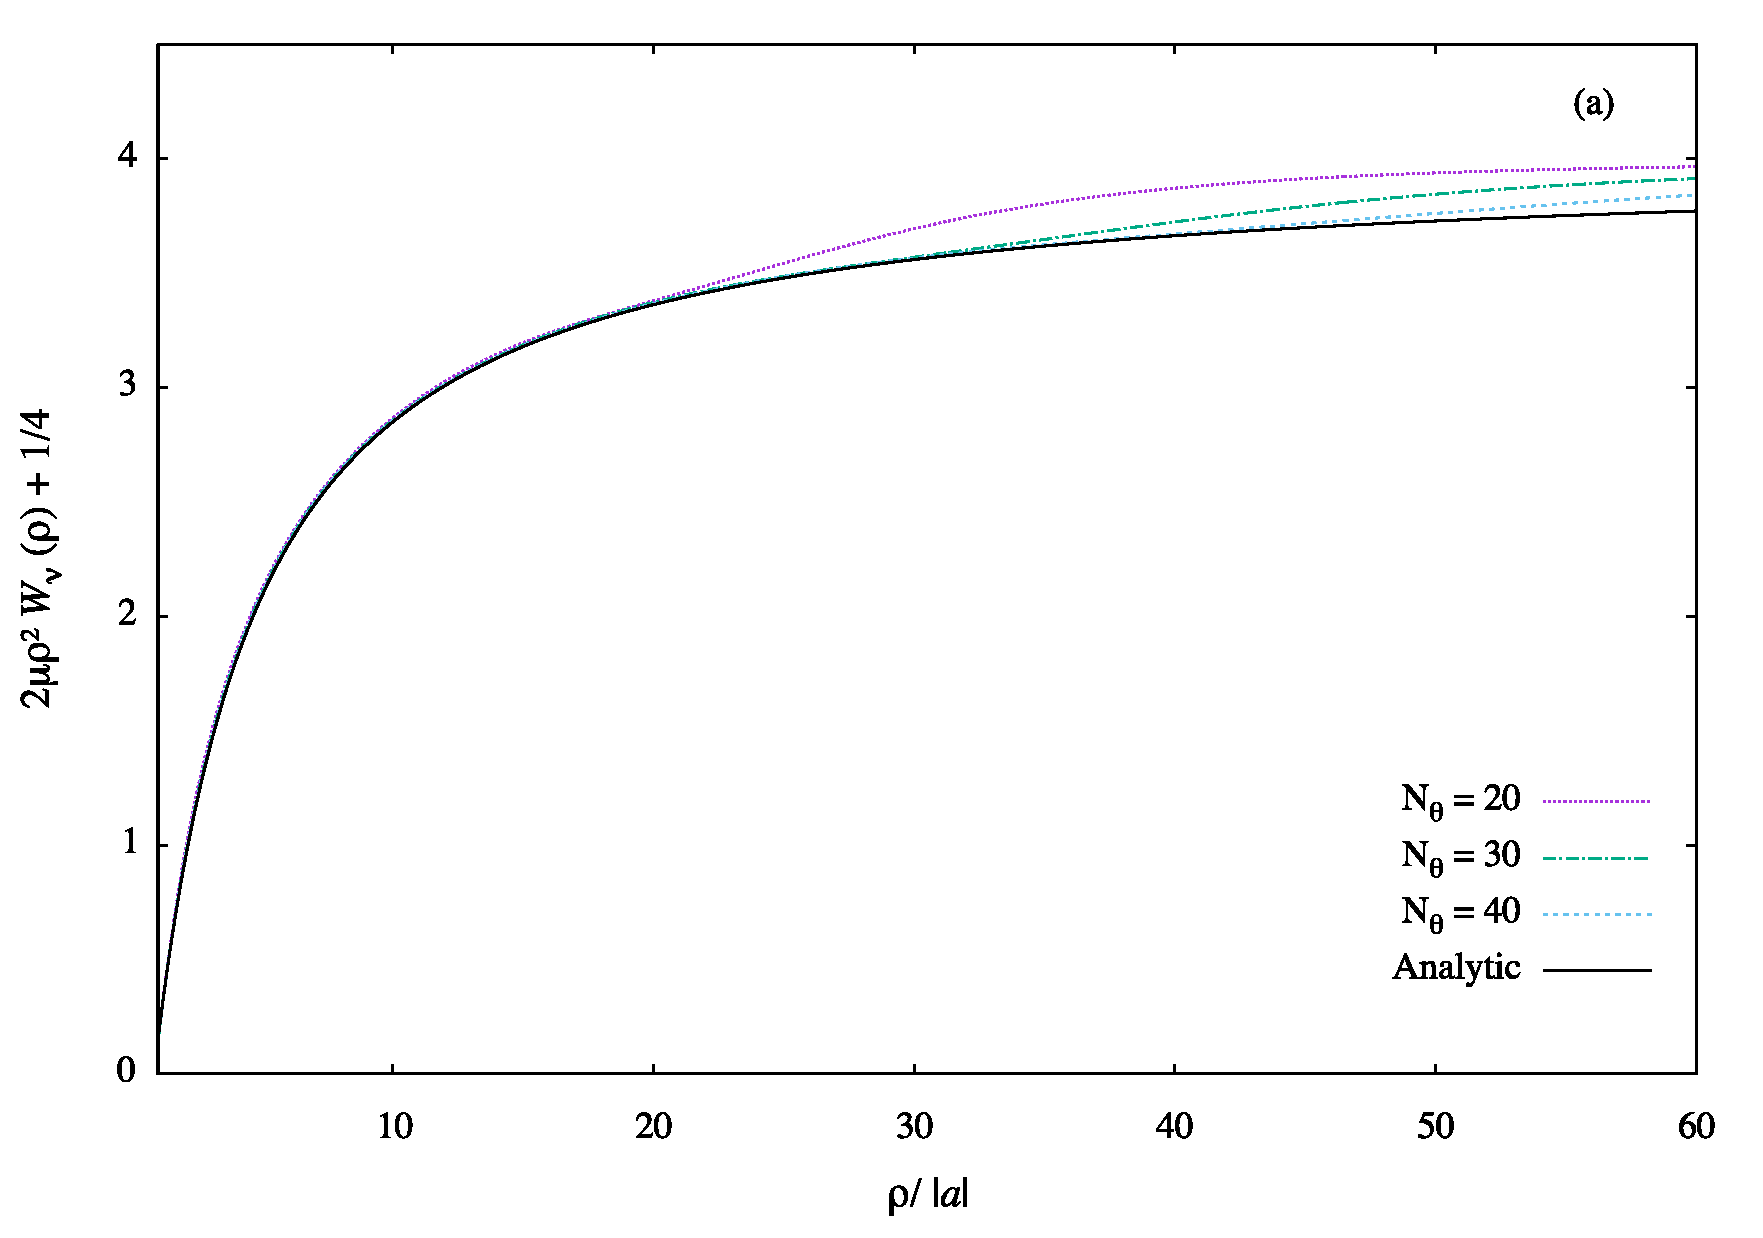
\includegraphics[width=1\linewidth]{convergence2.pdf}\label{fig:conv_2}}

	\subfigure[]{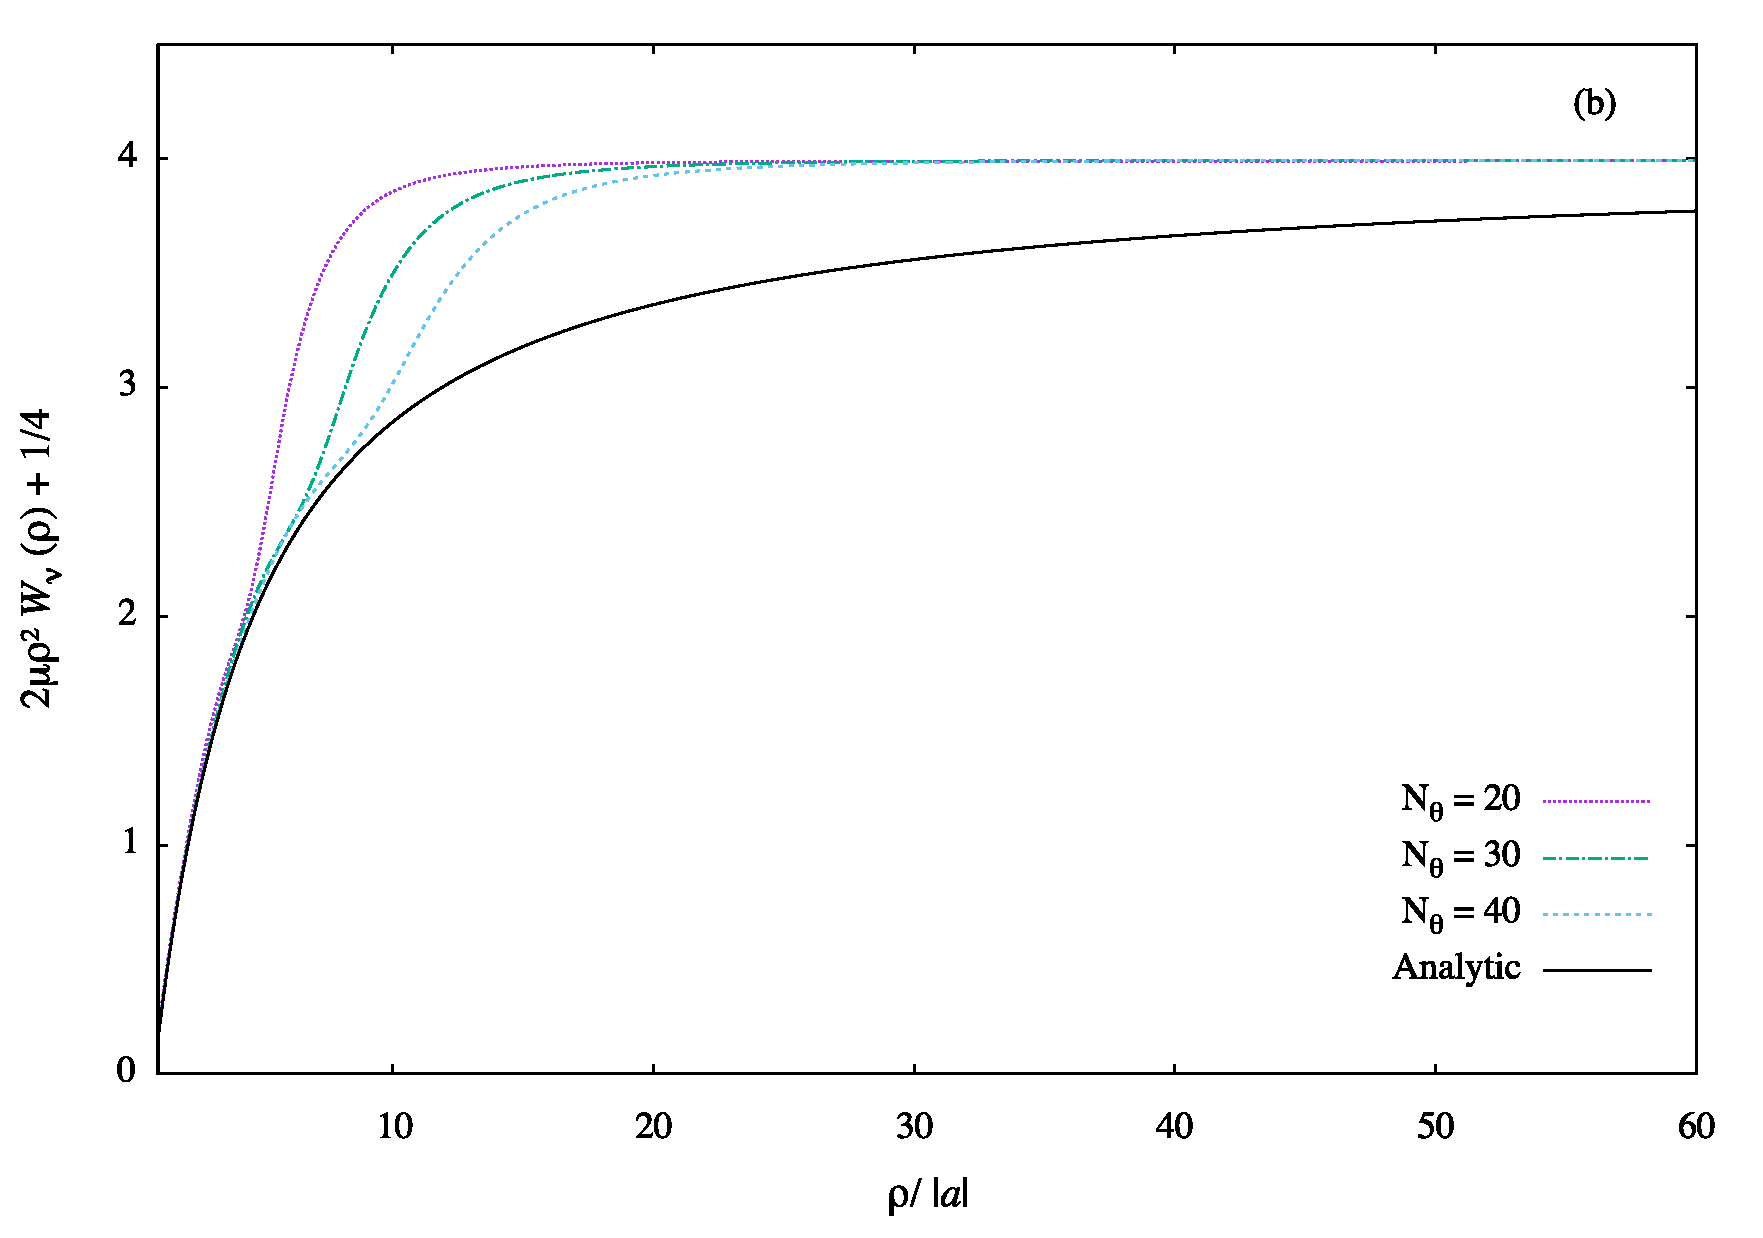
\includegraphics[width=1\linewidth]{convergence8.pdf}\label{fig:conv_8}} 
	\caption{Three-body effective potentials $\xi(\rho)$ for (a) $a_1=-2385$ a.u. and (b) $a_2=-8720$ a.u. plotted as functions of $\rho/\abs{a}$. The potentials, calculated using an increasing number of B-splines, are shown together with the eigenvalues $\nu_0(\rho/\abs{a})$ of \Cref{eq:faddeev_hyperang} for $a<0$.}
	\label{fig:conv}
\end{figure}

The calculations for positive $a$ were performed with an increasingly refined mesh, using the same hyperradial grid as in the calculations for $a<0$. In \Cref{fig:conv_pos1} we show the effective three-body potentials $\xi(\rho)$ for $a=1018$ a.u., plotted as functions of $\rho/\abs{a}$, together with the eigenvalues $\nu_0(\rho/\abs{a})$ for $a>0$. Here we observe that the convergent behaviour of $\xi(\rho)$ deviates from the effective potential $\nu_0(\rho/\abs{a})$. The slightly different form in the parabolic divergency of the curves is due to a discrepancy between the exact two-body energy $E_{2b}$, which is given in \Cref{eq:exact_2b}, and the energy of the universal shallow dimer $-E_D=-1/ma^2$. To illustrate this more clearly we have written the adiabatic potential $\nu_0(\rho)$ on the form  

\begin{equation}
\widetilde{W}(\rho) =\frac{\nu_0(\rho)-1/4}{2\mu \rho^2},
\end{equation}
and plotted this effective three-body Faddeev potential, together with the numerically calculated three-body effective potentials $W_{\nu}(\rho)$, as functions of $\rho/a$ in \Cref{fig:twobody}. The numerical potentials can be seen to converge to the exact energy of the binary subsystem (a dashed black line marked $E_{2b}$ in the figure), while the Faddeev potential approaches the approximate energy of the universal dimer (a dashed black line marked $-E_D$ in the figure). Since the binding energy of the universal energy is exact in the resonant limit $a \rightarrow \infty$, we expect a reduced discrepancy between the analytic and the numerical curves as $a$ is increased. In \Cref{fig:conv_pos5} we show that the potential curves for $a=5655$ a.u. converging as the number of B-splines are increased to 

\begin{figure}
	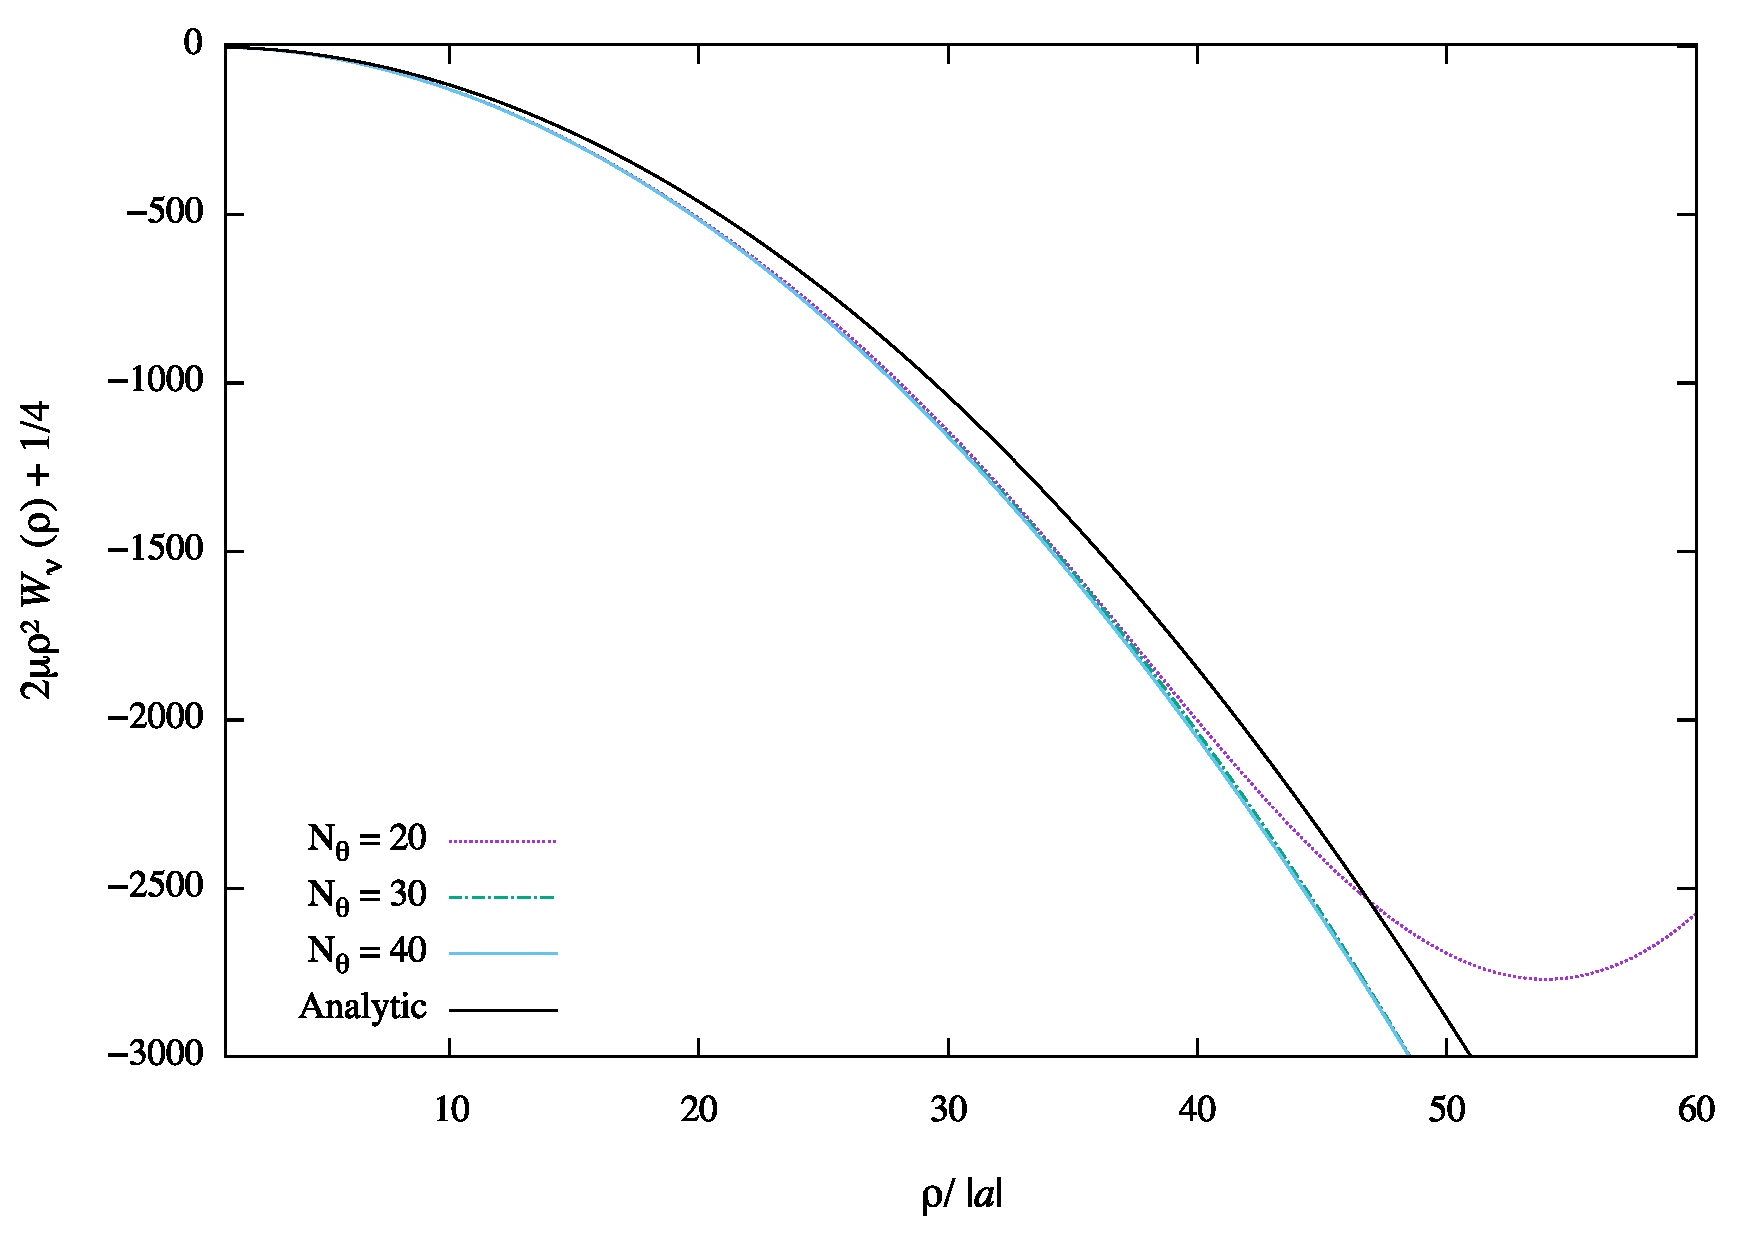
\includegraphics[width=\linewidth]{convergence1.pdf}
	\caption{Three-body effective potentials $\xi(\rho)$ for $a=1018$ a.u., plotted as functions of $\rho/\abs{a}$, are shown together with the eigenvalues $\nu_0(\rho/\abs{a})$ of \Cref{eq:faddeev_hyperang} for $a>0$. The numerically calculated potentials can be seen to converge to a slightly different form than $\nu_0(\rho/\abs{a})$.}
	\label{fig:conv_pos1}
\end{figure}

\begin{figure}
	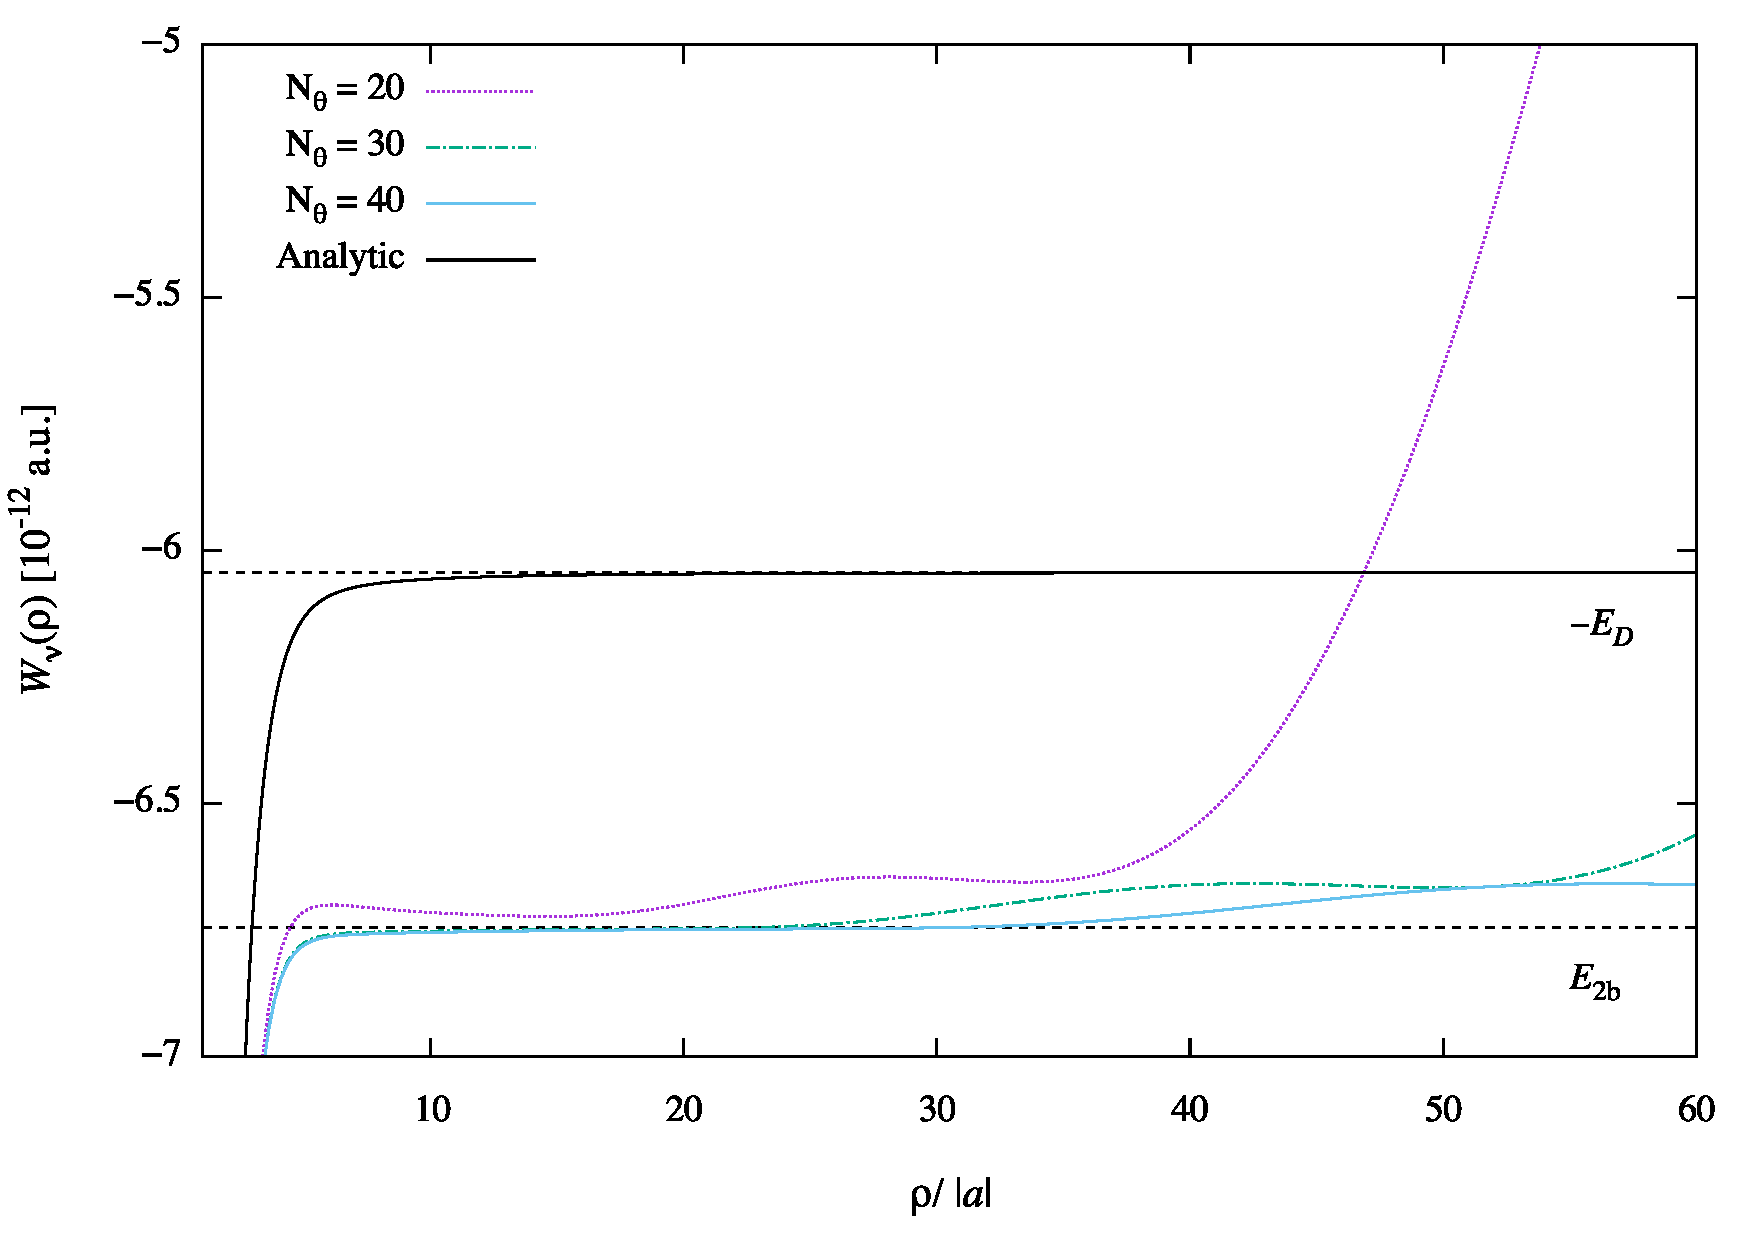
\includegraphics[width=\linewidth]{twobodyenergy.pdf}
	\caption{}
	\label{fig:twobody}
\end{figure}

\begin{figure}
	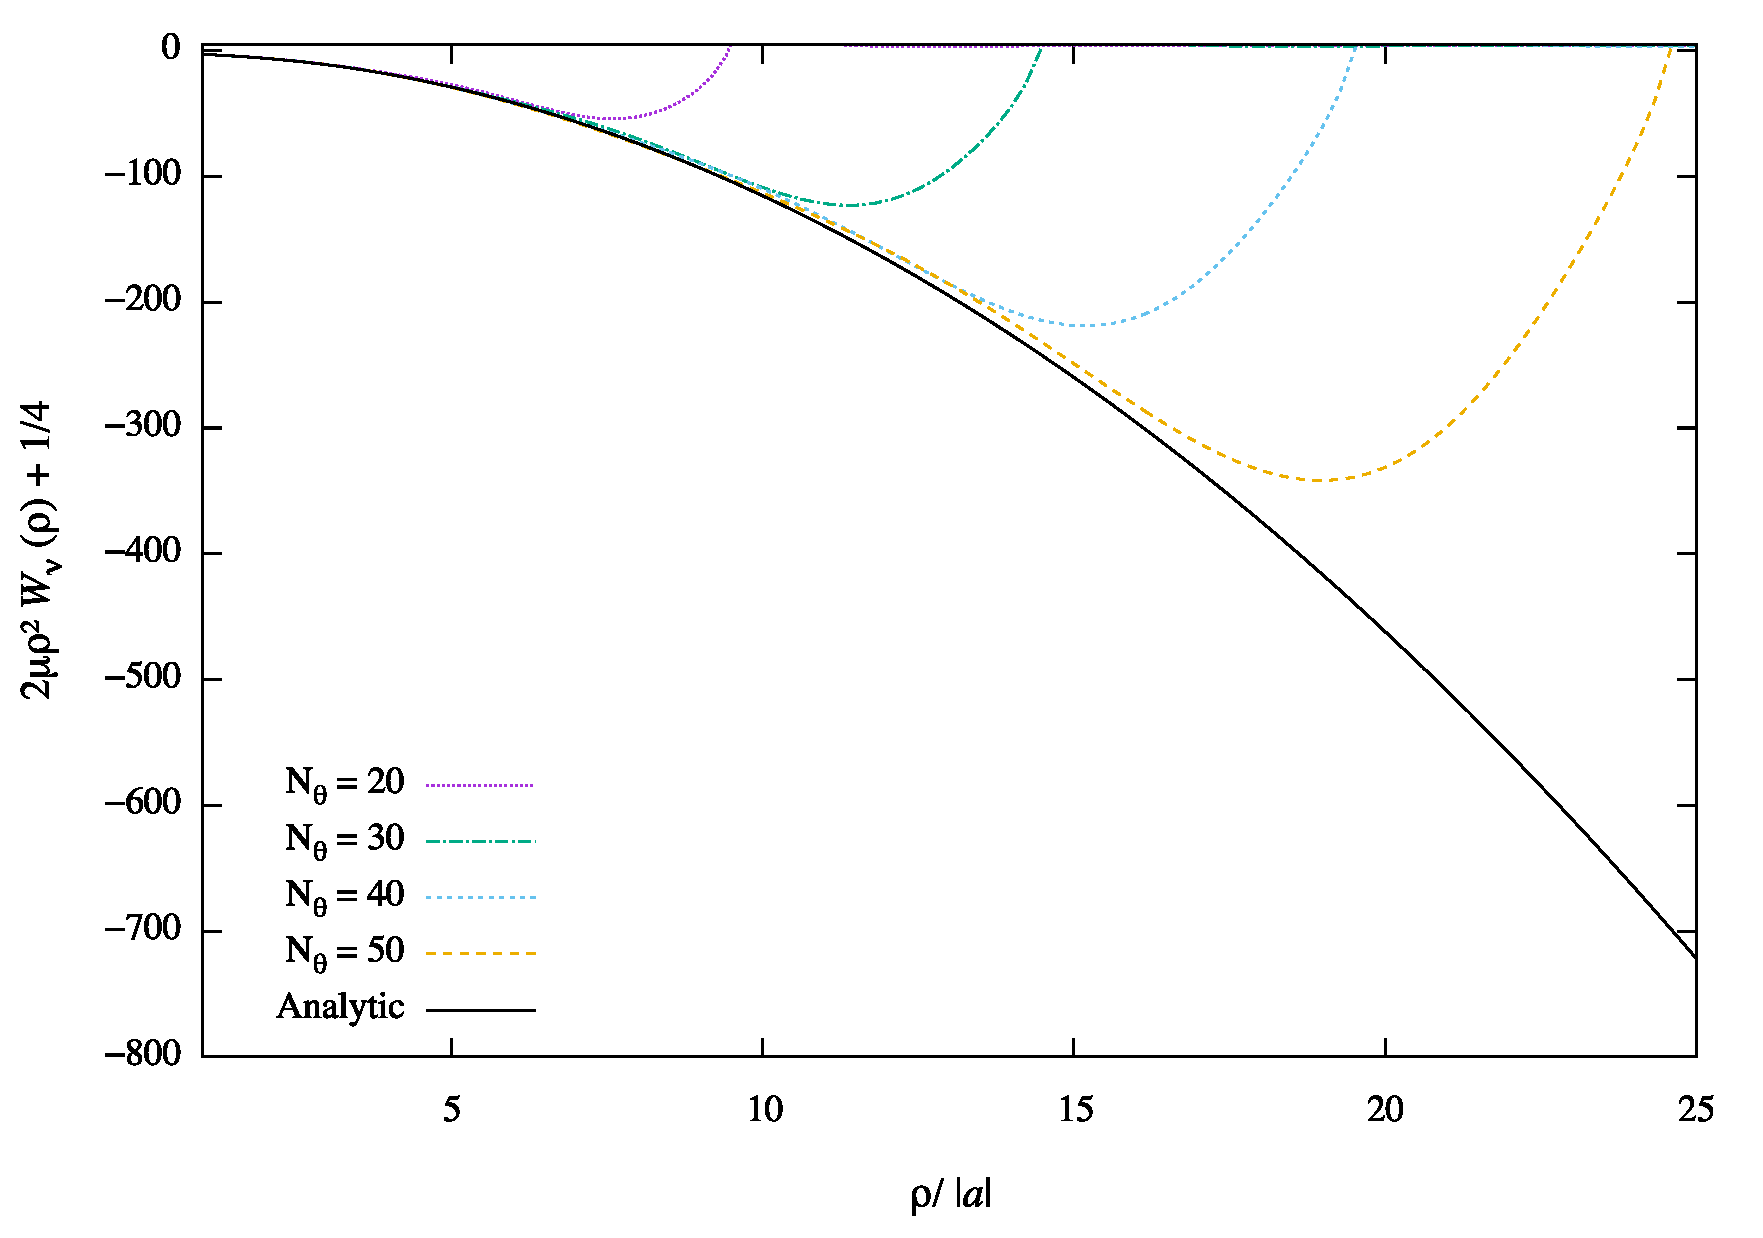
\includegraphics[width=\linewidth]{convergence5.pdf}
	\caption{The convergence toward the analytically derived eigenvalues $\lambda_0$ for $a=5655$ a.u. is shown for several different numbers of mesh points $N_{\theta}=N_{\phi}$.}
	\label{fig:conv_pos5}
\end{figure}


The hyperradial range for convergence is larger for the state with smaller $\abs{a}$, we suspect that this discrepancy is due to the knot point placement but this has not been verified yet. 
at for the hyperangular Further computational improvements must be imple- mented. This is a reasonable result since the convergence towards $-s_0^2$ is expected in the intermediate region $r_0 \gg \rho \gg \abs{a}$ and numerical difficulties aries at large $\rho$  



%"To get a better understanding of the connection of the recombination resonance shown in
%Fig. 1 to the Efimov effect, it is useful to examine the approximate adiabatic hyperspherical
%potentials sketched in Fig. 2. These potentials were constructed following the description given
%previously. In particular, for the region r0 ≪ R ≪ |a|, the lowest three-body breakup channel
%(labeled α in the figure) has the attractive 1/R2
%character predicted by Efimov. The key
%observation is that for a < 0, there is a barrier in the initial free atom channel. Just as with any
%barrier, it is possible to have a resonance. In this case, it is a three-body shape resonance. In a
%normal collision, the potentials are fixed, and the collision energy is varied to reveal the resonant
%behavior. Since the collision energy is fixed by the temperature in an ultracold gas, however, we
%must scan the scattering length to see the resonance. As the scattering length is changed, the
%position of the barrier grows proportional to |a|; and its height, to 1/a2
%. The resonance energy
%thus decreases as |a| increases and at some particular a will coincide with the collision energy,
%giving the observed resonance. The recombination rate is enhanced when this happens because
%the amplitude of the scattering wave function behind the barrier — where the coupling to the
%atom-dimer channel peaks — grows much larger on resonance."

In the following we will look closer into the structure of the Efimov-like potentials $W_{\nu}$ for finite $a$. The adiabatic potential curves were here numerically calculated with a potential strong enough to support a single $s$-wave bound states and the potential depth $d$ was tuned to yeild a scattering length of $a=228$ a.u. The adiabatic potential curves $W_{\nu}$ with $\nu = 0-4$ are plotted as functions of the hyperradius $\rho/a$. In this figure we can see that the lowest potential curve $\nu = 0$ are converging to the two-body $s$-wave binding energy, which represent channels with one two-body bound state and a free particle. Here the channel index $\nu=1$ corresponds to the Efimov channel. The higher lying channels $\nu>1$ are continuum channels and the channel index $\nu=0$ represents a deeply bound state.

\begin{figure}
	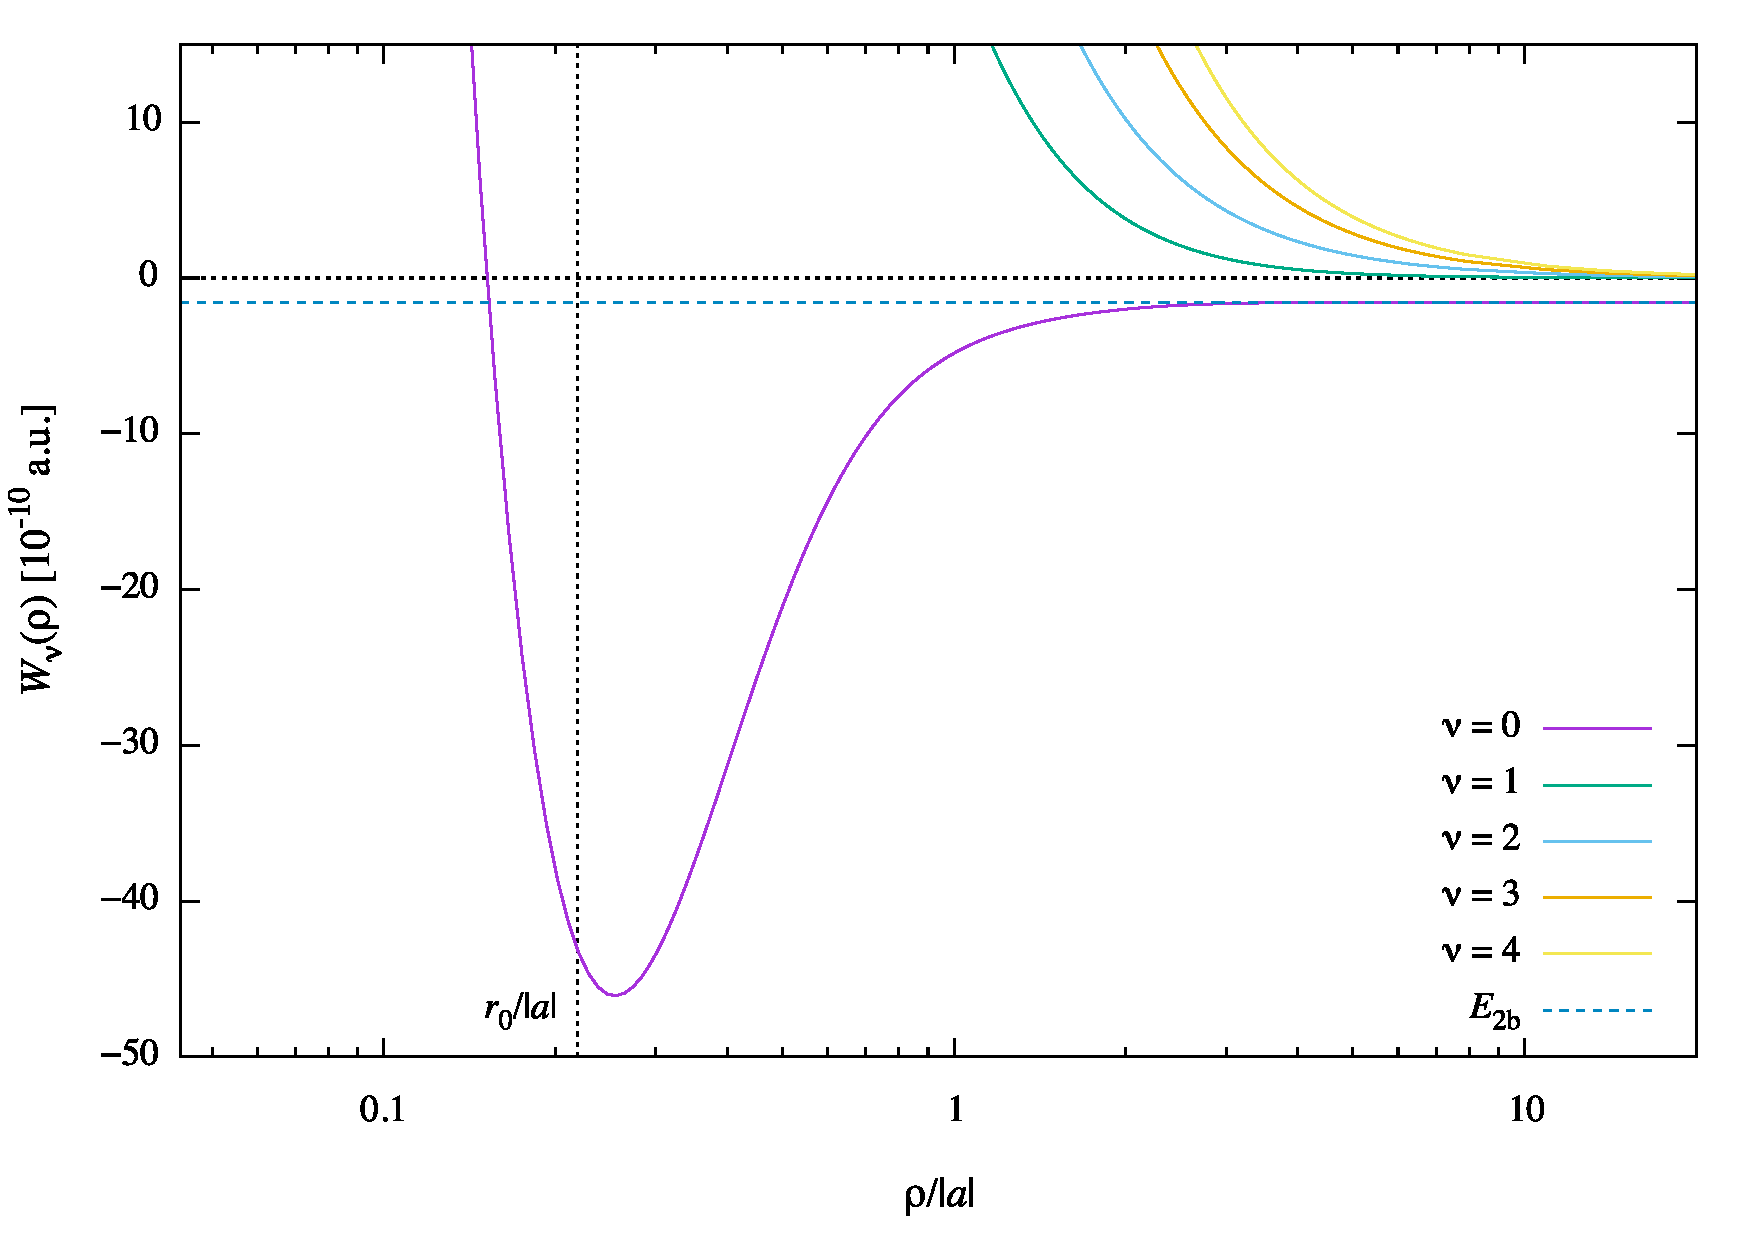
\includegraphics[width=\linewidth]{Wpos2.pdf}
	\caption{Three-body effective potentials for $a>0$. The horizontal dashed line is $-s_0^2$.}
	\label{fig:Wpos}
\end{figure}

\begin{figure}
	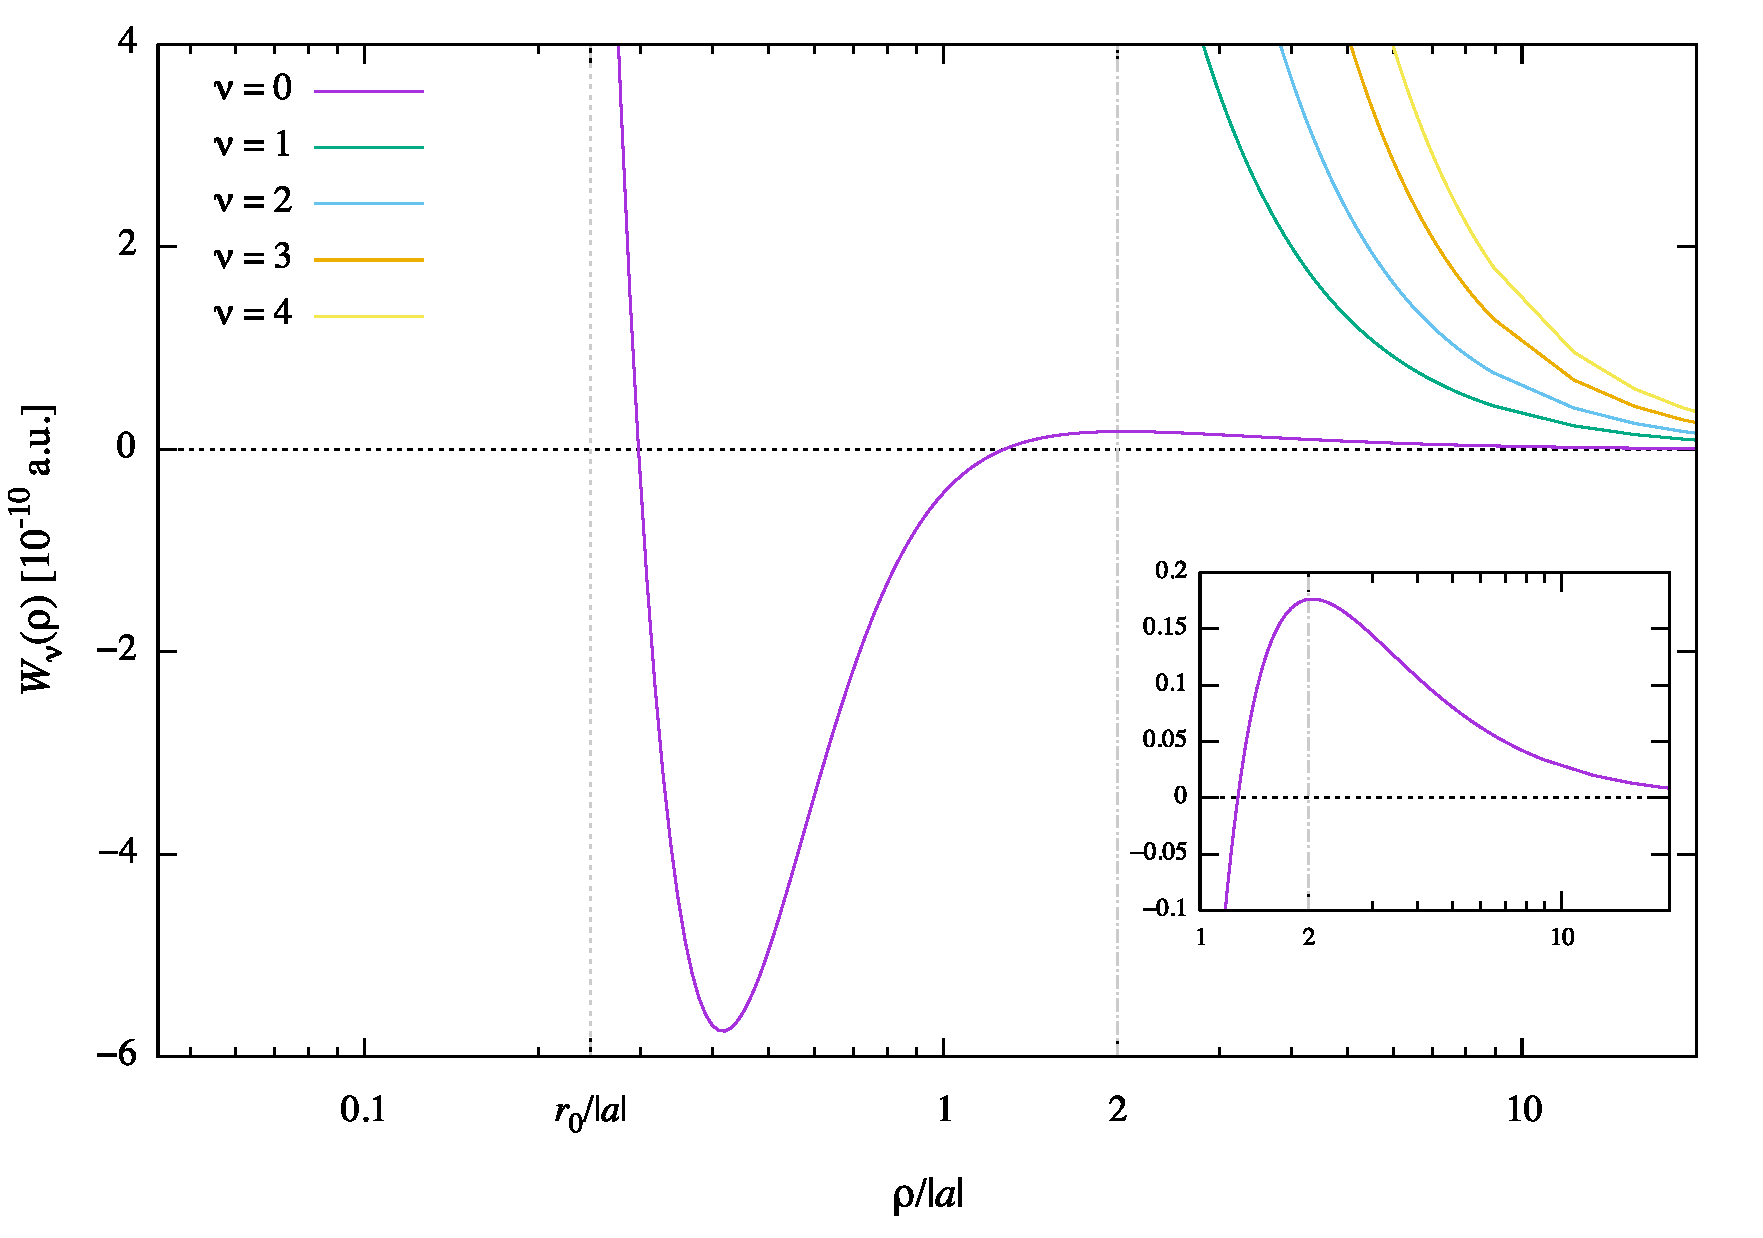
\includegraphics[width=\linewidth]{Wneg2.pdf}
	\caption{Three-body effective potentials for $a>0$. The horizontal dashed line is $-s_0^2$.}
	\label{fig:Wneg}
\end{figure}

For all results presented above we were able to acheive convergence using a uniformly spaced mesh for hyperradii up to $\rho \approx 5000$ a.u. However, at larger hyperradii the two-body potential surface $V(\rho,\theta,\phi)$ changes much more rapidly near the coalescence points, i.e., at the hyperangular configurations $(\theta,\phi) = (\pi/2,\phi)$, $(\pi/2,\phi - 2\pi/3)$ and $(\pi/2,\phi - 2\pi/3)$. In \Cref{fig:surfaces} the two-body potential surfaces are plotted at two different hyperradii to illustrate how the size of the system changes the numerical complexity. To account for the increased numerical difficulties with increasing system size, the grid was more densly packed near the boundary $(\theta,\phi)=(\pi/2,\pi/3)$ for $\rho > 5000$. 

\begin{figure}
	\centering  
	\subfigure[The potential surface for $\rho=r_0$.]{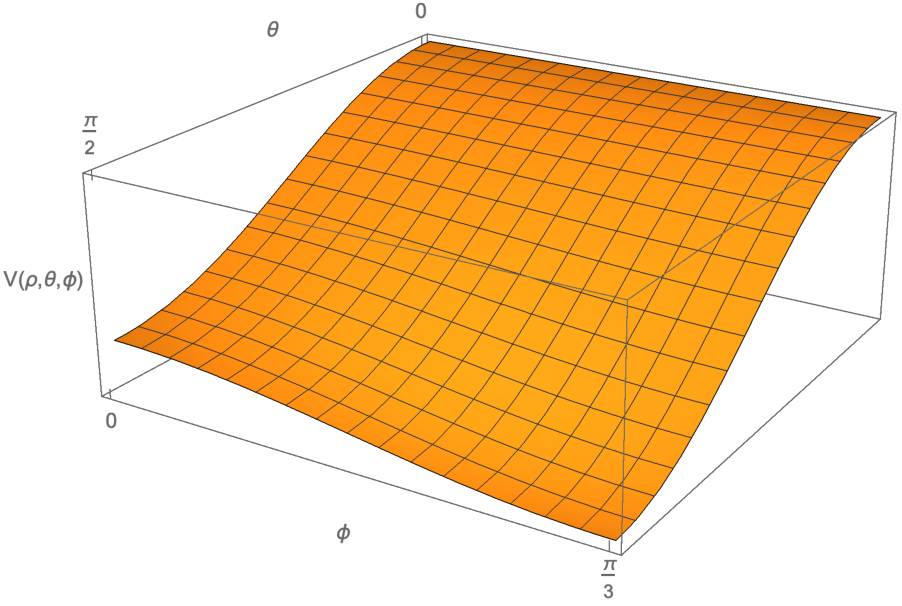
\includegraphics[width=0.45\linewidth]{surface_small.pdf}}
	\subfigure[The potential surface for $\rho=3r_0$.]{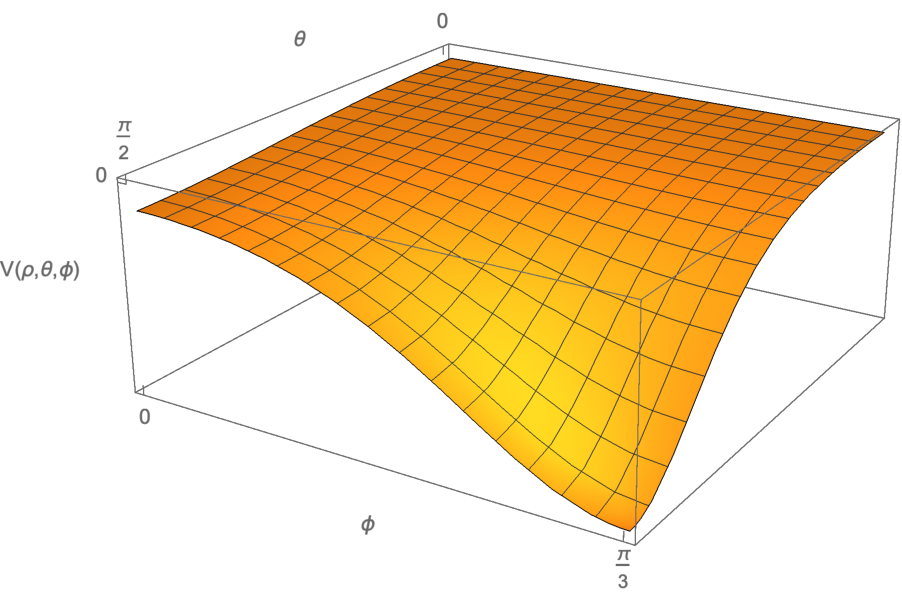
\includegraphics[width=0.45\linewidth]{surface_large.pdf}}
	\caption{Illustration of the two-body potential surfaces at two different hyperradii $\rho$. The potential surface change more rapidly at the hyperangular configuration $(\theta,\phi)=(\pi/2,\phi)$ for larger $\rho$.}\label{fig:surfaces}
\end{figure}

